% chap2.tex

\chapter{MiniBloq}\label{chap:minibloq}
This chapter disucusses the design and enhancement of the visual programming environment MiniBloq for robotic platform.

\section{Introduction}
MiniBloq is a graphical development environment for Arduino and other platforms. Its main objective is to help in teaching programming using a drag and drop blocks called Action blocks. It is specially used at elementary, middle and high schools. The MiniBloq version v0.82 used in this research comes only in Windows version, since the Linux is under development.

\section{Enhancement for robotic platform}
Minibloq is a graphical code generator with IDE capabilities. It's self-contained and every distribution includes the complete tools needed to compile (or interpret, depending on the selected target) and deploy the code to the selected hardware target. Every code block is configured in XML. To solve a given problem, the blocks are arranged in a logical manner and then the compiled executable file is transferred to the hardware via data cable. An advantage of Minibloq compared to other graphical programming softwares is that it can be enhanced to add new blocks with functionality specific to your hardware.

MiniBloq is specifically enhanced for Electric Ray robot by adding new blocks by abstracting the pin level details of the hardware. Thus, various blocks for for controlling movement, sensors, display and buzzer of Electric Ray Robot are available to program. The new blocks developed is shown in the Figure~\ref{fig:blocks}. The enhanced interface of MiniBloq is shown in Figure ~\ref{fig:graphical}.

\begin{figure}[h]
\centering
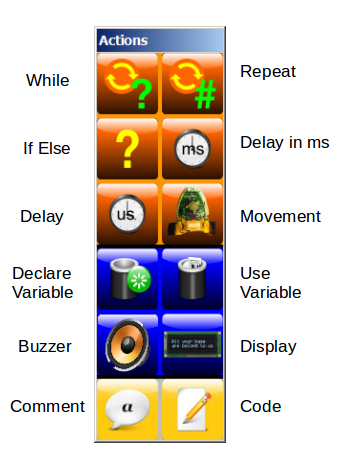
\includegraphics[width=0.45\columnwidth]{Images/minibloq-blocks}
\caption{New blocks developed for Electric Ray}
\label{fig:blocks}
\end{figure}

\begin{figure}[h]
\centering
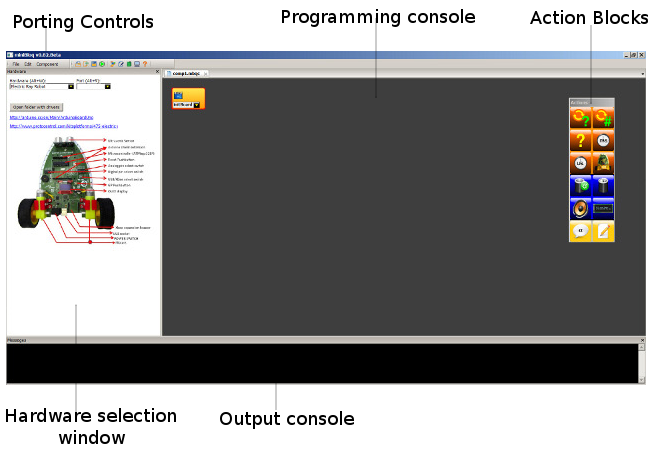
\includegraphics[width=1\columnwidth]{Images/minibloq}
\caption{Enhanced Minbloq programming environment for Electric Ray}
\label{fig:graphical}
\end{figure}

The blocks are designed to be intuitive. A "Hello World" program in the developed graphical tool is written by dragging and droping a block for OLED display, followed by text in the form of string literal as shown in the Figure~\ref{fig:helloworld}. The program when ported to the Electric Ray robot will display the string "Hello World" in OLED.

\begin{figure}[h]
\centering
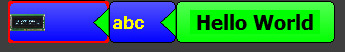
\includegraphics[width=0.5\columnwidth]{Images/minibloq-helloworld}
\caption{Hello World program in Minibloq}
\label{fig:helloworld}
\end{figure}

Internally the programming environment converts building blocks to its corresponding C++ 
code compatible with Arduino. Students interested in modifying the existing property of the building block are allowed to edit the generated C code. For example a code generated for forward movement in the form of block is shown in the Figure~\ref{fig:code}.

\begin{figure}[h]
\centering
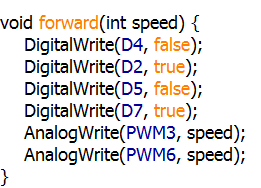
\includegraphics[width=0.35\columnwidth]{Images/minibloq-code}
\caption{Code generated for forward block}
\label{fig:code}
\end{figure}

Connect the robot using a data cable and choose the connected port in MiniBloq interface. Click on the green play button at the top. This will compile the program and port the program to the robot. A detailed manual on the blocks and is made available at Appendix ~\ref{apdx:a}

